
\documentclass{article}
\usepackage[utf8]{inputenc}
\usepackage{amsthm}
\usepackage{amsmath, mathtools, amsfonts,amssymb}
\usepackage{graphicx}
\usepackage{verbatim}
\usepackage{fancyhdr}
% Code
\usepackage{listings} 
\usepackage{algorithm}
\usepackage{algpseudocode}
% Margins
\usepackage{geometry}
%\usepackage{enumitem} % for nice enumerating
\geometry{margin=1in}

% Graphics
\usepackage{tikz}
\usetikzlibrary{matrix} % matrices
\usepackage{tikz-qtree} % Simple trees
\usepackage{verbatim} % what is this for again???

\setcounter{section}{-1}

\newtheorem{pic}{Figure}
\numberwithin{pic}{section}
\newtheorem{lem}{Lemma}
\numberwithin{lem}{section}
\newtheorem{thm}{Theorem}
\numberwithin{thm}{section}
\newtheorem{cor}{Corollary}
\numberwithin{cor}{section}

\theoremstyle{definition}
\newtheorem{ex}{Example}
\numberwithin{ex}{section}
\newtheorem{defn}{Definition}
\numberwithin{defn}{section}
\theoremstyle{definition}
\newtheorem{prob}{Problem}

\theoremstyle{remark}
\newtheorem*{con}{Conjecture}
\newtheorem{rem}{Remark}
\newtheorem*{cex}{Counterexample}
\newtheorem*{ts}{T.S.}

%%% COMMANDS %%%
% Sets
\newcommand{\set}[1]{\ensuremath{\left\{ #1\right\}}} % write sets
\newcommand{\e}{\ensuremath{\epsilon}} % Epsilon
\newcommand{\R}{\ensuremath{\mathbb{R}}} % Real Numbers
\newcommand{\N}{\ensuremath{\mathbb{N}}} % Natural numbers
\newcommand{\Q}{\ensuremath{\mathbb{Q}}} % Rationals
\newcommand{\I}{\ensuremath{\mathbb{I}}} % Irrational Numbers
\newcommand{\Z}{\ensuremath{\mathbb{Z}}} % Integers
% Easier Delimiters?
\newcommand{\lr}[2]{\ensuremath{\left#1 #2 \right #1}}
% Absolute Value
\newcommand{\abs}[1]{\ensuremath{\left| #1 \right|}}
% Landau Notation
\newcommand{\Oh}{\ensuremath{\mathcal{O}}} %%% IN MATH MODE
\newcommand{\oh}{\ensuremath{\mathcal{o}}} %%% IN MATH MODE
% Display style fractions
\newcommand{\Frac}[2]{\displaystyle \frac{#1}{#2}}
% Display style limits
\newcommand{\Lim}[2]{\displaystyle \lim_{#1}{#2}}

% Enumerate
\renewcommand{\labelenumi}{(\alph{enumi})}
\renewcommand{\labelenumii}{\roman{enumii}}

% change proof environment
\renewcommand*{\proofname}{Pf}

% Indentation
\newlength\tindent
\setlength{\tindent}{\parindent}
\setlength{\parindent}{0pt}
\renewcommand{\indent}{\hspace*{\tindent}}

% Set title
\title{X}

\begin{document}


\fancyhead[l]{Quinn Stratton}
\fancyhead[c]{Nate CS Assignment One}
\fancyhead[r]{\today}
\pagestyle{fancy}


\begin{prob}
  Go to the terminal application and make a new directory to store code. Inside this directory make another for this assignment. Add a \textit{readme} file to this directory.
\end{prob}

\begin{prob}
  Write a \textit{C} program to read in a number, and then display some silly math facts about that number, i.e. $x$ times 7 is $y$, $x^2$ is $z$, etc. Add this program to github.
\end{prob}

\begin{prob}
  Write a \textit{C} program that takes in two integers and outputs the division algorithm performed with those two numbers as inputs. Add that program to github. Below is an example of output.\\
  \begin{center}
    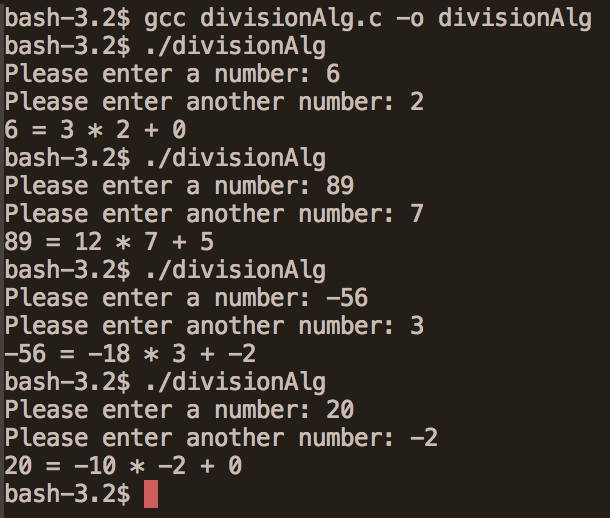
\includegraphics[scale=0.5]{soln1}
  \end{center}
\end{prob}

\begin{prob}
  DeMorgan's laws state that
  \begin{align}
    \neg(P \vee Q) &\iff \neg P \wedge \neg Q\\
    \neg(P \wedge Q) &\iff \neg P \vee \neg Q
  \end{align}
  Prove one of these identities by way of a truth table.
\end{prob}

\begin{prob}
  Consider the following recursively defined function,
  $$f(n) =
  \begin{cases}
    1 &\text{if }n \leq 1\\
    n\cdot f(n / 2) &\text{if }n\mod 2 = 0\\
    n + f(n - 1) &\text{if }n\mod 2 = 1
  \end{cases} $$
  Calculate $f(20)$.
\end{prob}

\begin{prob}
  Let $a,b$ be characters, $\epsilon$ be the empty string, and $\circ$ denote string concatenation. Consider the following definition of a $foo$,
  $$foo =
  \begin{cases}
    \epsilon\\
    a\circ foo \circ a\\
    a\circ foo \circ b\\
    b\circ foo \circ a\\
    b\circ foo \circ b
  \end{cases}
  $$
  \begin{enumerate}
  \item Is $aba$ a $foo$?
  \item Is $babb$ a $foo$?
  \item In more intuitive terms, what is a $foo$?
  \end{enumerate}
\end{prob}

\begin{prob}
  A \textit{Triangular Number} counts objects that are arranged into equilateral triangles (see the image below, lifted from Wikipedia).\\
  \begin{center}
    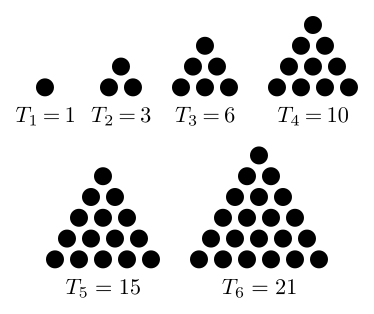
\includegraphics[scale=0.5]{TriNums}
  \end{center}
  \begin{enumerate}
  \item Come up with a recursive definition for $T_n$, the $n^{th}$ triangular number.
  \item Come up with a non-recursive formula for $T_n$ (extra credit: prove this formula via induction).
  \item Let $S_n$ denote the sequence of non-zero perfect squares, i.e. $S_1 = 1, S_2 = 4, S_3 = 9, ...$. Prove that $S_n = T_n + T_{n-1}$ for $n \geq 2$. \textit{Hint:} the closed formula from part (b) may be helpful, bonus if you can also devise a ``proof by picture''.
  \end{enumerate}
\end{prob}
\end{document}